\section{Resonances}

To describe the complicated behaviour of cross sections, we must use some model for their behaviour. The classical model is the \textbf{Single Level Breit-Wigner} (SLBW) formalism. This is sufficient for our purposes, but has now been largely superseded by the Multi Level Breit-Wigner or Reich-Moore (pronounced Rich-More) formalism in practical applications.

We will begin by making some definitions. Resonances can be characterised by their location in energy, $E_0$, the peak value for the total cross section, $\sigma_0$, and their `channel width', $\Gamma$, or the energy interval it spans between the two points at half the maximum values (otherwise known as the Full Width at Half Maximum, FWHM). The main components of a SLBW resonance are illustrated in Fig.~\ref{fig:resSLBW}.

For the (n,$\gamma$) reaction, SLBW gives:
\begin{equation*}
    \sigma_\gamma(E_\mathrm{CM}) = \sigma_0 \frac{\Gamma_\gamma}{\Gamma}\left(\frac{E_0}{E_\mathrm{CM}}\right)^{\frac{1}{2}}\frac{1}{1+y^2}\;\mathrm{,}
\end{equation*}
where:
\begin{equation*}
    E_\mathrm{CM} \equiv \text{neutron energy in Centre of Mass frame}\;\mathrm{,}
\end{equation*}
(note $E = E_\mathrm{LAB} = \frac{A+1}{A}E_\mathrm{CM}$)
\begin{equation*}
    E_0 \equiv \text{energy of the resonance}\;\mathrm{,}
\end{equation*}
\begin{equation*}
    y = \frac{2}{\Gamma}(E_\mathrm{CM} - E_0)\;\mathrm{,}
\end{equation*}
(at the resonance peak $E_\mathrm{CM} = E_0$ giving $\sigma_\gamma = \sigma_0 \frac{\Gamma_\gamma}{\Gamma}$),
\begin{equation*}
    \Gamma \equiv \text{total resonance width (FWHM)}\;\mathrm{,}
\end{equation*}
(this also has the quantum mechanical definition of $\Gamma = \hbar/\tau$, where $\tau$ is the average lifetime of a compound nucleus).
\begin{equation*}
    \Gamma_\gamma \equiv \text{radiative line width (partial width)}\;\mathrm{,}
\end{equation*}
\begin{equation*}
    \frac{\Gamma_\gamma}{\Gamma} \equiv \text{probability of decaying through the (n,}\gamma\text{) channel}\;\mathrm{,}
\end{equation*}
\begin{equation*}
    \sigma_0 \equiv \text{total cross section at }E_\mathrm{CM}=E_0\;\mathrm{.}
\end{equation*}
There is also an equation for $\sigma_0$ which is:
\begin{equation*}
    \sigma_0 = 4\pi\lambdabar^2_0\frac{\Gamma_\mathrm{n}}{\Gamma}g\;\mathrm{,}
\end{equation*}
where:
\begin{equation*}
    \Gamma_\mathrm{n} \equiv \text{neutron emission line width}\propto E^\frac{1}{2}_\mathrm{CM} \;\mathrm{,}
\end{equation*}
\begin{equation*}
    \lambdabar_0 \equiv \text{reduced wave length corresponding to }E_0 = \frac{\hbar}{\sqrt{2\mu E_0}}\;\mathrm{,}
\end{equation*}
\begin{equation*}
    \mu \equiv \text{reduced mass} = \frac{A}{A+1} = \frac{mM}{m + M}\;\mathrm{,}
\end{equation*}
\begin{equation*}
    g \equiv \text{statistical factor} = \frac{2J+1}{(2S+1)(2I+1)}\;\mathrm{,}
\end{equation*}
where $S=\frac{1}{2}$ is the neutron spin, $I$ is the target nucleus spin ($I=0$ for even-even nuclides), and $J$ us the spin of the compound nucleus ($J = I - \frac{1}{2}$ or $J = I + \frac{1}{2}$). %The peak cross section can also be written as:
%\begin{equation*}
%    \sigma_0 \approx 2.608\times 10^6 \times \left(\frac{A+1}{A}\right)^2 \frac{1}{E_0 \text{(eV)}}\frac{\Gamma_\mathrm{n}}{\Gamma}g\;\mathrm{.}
%\end{equation*}
Note that if $E_\mathrm{CM}<< E_0$ and $A\rightarrow\infty$ (or $E << E_0$) then
\begin{equation*}
    \sigma(E) \sim \frac{1}{\sqrt{E}} \sim \frac{1}{v}\;\mathrm{.}
\end{equation*}

\begin{figure}[h!]
  \centering
  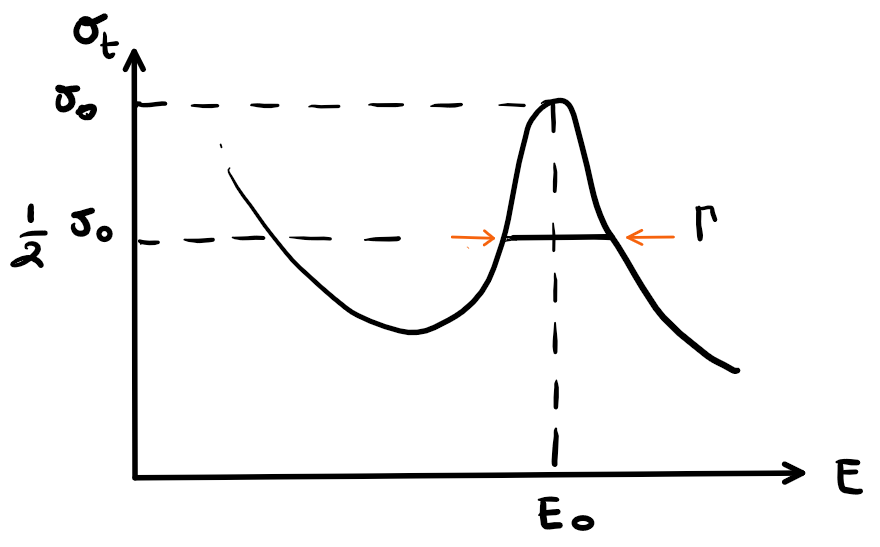
\includegraphics[scale=0.60]{./Figures/P3/slbw.png} 
  \caption{Illustration of a Single-Level Breit Wigner resonance.} 
  \label{fig:resSLBW}
\end{figure}

Scattering resonances are slightly more complicated. They have two additional terms: one due to potential scattering (nuclides behaving like hard spheres) and one due to interference effects -- we will leave it as quantum weirdness without further explanation.
\begin{equation*}
    \sigma_\mathrm{s}(E_\mathrm{CM}) = \underbrace{\sigma_0\frac{\Gamma_\mathrm{n}}{\Gamma}\left(\frac{E_0}{E_\mathrm{CM}}\right)^{\frac{1}{2}}\frac{1}{1+y^2}}_{\text{resonance scattering}} + \underbrace{\sigma_0 \frac{2R}{\lambdabar_0}\frac{y}{1+y^2}}_{\text{interference scattering}} + \underbrace{4\pi R^2}_{\text{potential scattering}}\;\mathrm{.}
\end{equation*}
Here $\Gamma_\mathrm{n}$ is the scattering channel width (or neutron width in literature) and $R$ is the nuclear radius $\sim r_0 A^\frac{1}{3} = 1.25\times 10^{-13}\times A^{\frac{1}{3}}$ cm.

\begin{figure}[h]
  \centering
  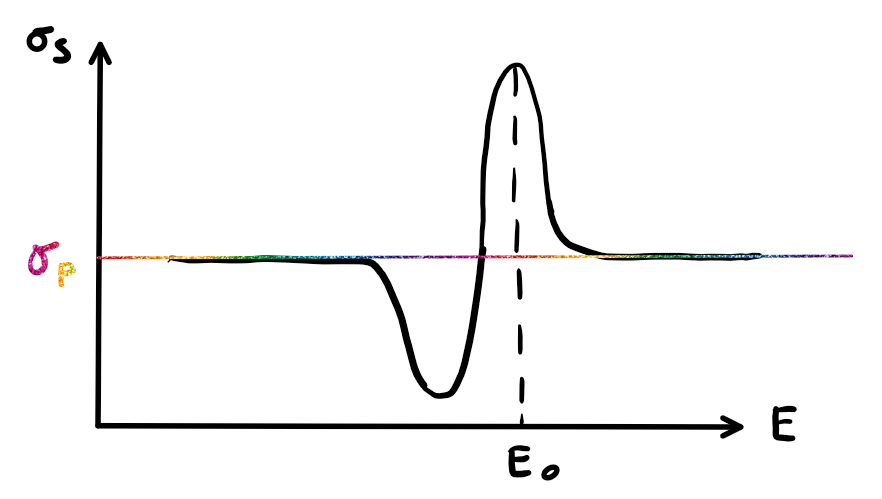
\includegraphics[scale=0.60]{./Figures/P3/slbwScatter.png} 
  \caption{Illustration of a scattering resonance.} 
  \label{fig:res}
\end{figure}

Potential scattering is independent of energy. In a mixture, the sum of the potential scattering cross sections of all nuclides results in a `background' cross section. If this background cross section is sufficiently high, it will drown out resonances -- they will be submerged under this background cross section. This is important with respect to determining how strongly a resonance affects the flux spectrum. %We talk about the practical width of a resonance, $\Gamma_\mathrm{prac}$, which measures the extent to which a given resonance cross section extends above the background.
We will examine the relative strength of a resonance at its peak versus the total background cross section in the presence of a moderator. We will use p to denote the potential scatter cross section, A to denote an absorber, and H to denote the moderator (hydrogen). Given that $\Sigma_{\mathrm{A},\mathrm{peak}} = N_\mathrm{A}\sigma_{\mathrm{A},0}$, this can be written as:
\begin{equation*}
    \frac{\Sigma_{\mathrm{A},\mathrm{peak}}}{\Sigma_\mathrm{p}} = \frac{N_\mathrm{A}\sigma_{\mathrm{A},0}}{N_\mathrm{A}\sigma_{\mathrm{A},\mathrm{p}} + N_\mathrm{H}\sigma_{\mathrm{H},\mathrm{p}}} = \frac{\sigma_{\mathrm{A},0}}{\sigma_{\mathrm{A},\mathrm{p}} + \frac{N_\mathrm{H}}{N_\mathrm{A}}\sigma_{\mathrm{H},\mathrm{p}}}\;\mathrm{.}
\end{equation*}
The quantity $\frac{N_\mathrm{H}}{N_\mathrm{A}}$ is referred to as the dilution. As $\frac{N_\mathrm{H}}{N_\mathrm{A}}\rightarrow \infty$, the relative importance of $\sigma_{\mathrm{A},0}$ (or the resonance) goes to 0. This case is commonly referred to as infinite dilution and means that the resonance does not perturb the neutron flux. More generally, dilution refers to the ratio of the resonance nuclide density to that of all other nuclides. Perhaps, more usefully, one also talks about the `background cross section', $\sigma_\mathrm{b} = \frac{\sigma_\mathrm{H,p}N_\mathrm{H}}{N_\mathrm{A}}$. Then one can phrase things in terms of the relative sizes of microscopic cross sections -- if there is a high background or a low background.

\subsection{Evaluating the resonance escape probability}

With this, we can evaluate the resonance escape probability we saw previously in Eq.~\eqref{eq:res_escape_prob} if we assume an SLBW form of the resonance and say that our absorber is infinitely dilute. Initially, this probability has the form:
\begin{equation*}
    p(E) = \exp{\left(-\int^{E_0}_E\frac{\Sigma_\mathrm{a}(E')}{\Sigma_\mathrm{s}(E') + \Sigma_\mathrm{a}(E')}\frac{\mathrm{d}E'}{E'}\right)} = \exp{\left(-\int^{E_0}_E\frac{N_\mathrm{A}\sigma^{\mathrm{A}}_\gamma(E')}{N_\mathrm{H}\sigma^\mathrm{H}_\mathrm{s} + N_\mathrm{A}\sigma^{\mathrm{A}}_\gamma(E')}\frac{\mathrm{d}E'}{E'}\right)}\;\mathrm{.}
\end{equation*}
We will make two approximations. First, we will say the absorber is infinitely dilute, i.e., $N_\mathrm{H}\sigma^\mathrm{H}_\mathrm{s} >> N_\mathrm{A}\sigma^{\mathrm{A}}_\gamma(E')$. Second, we will say contributions to the integral are small far away from the resonance (above or below), i.e., we are evaluating the integral in the small vicinity about $E_0$, the resonance energy, so we can write $\int_{E_0}\mathrm{d}E'$. This allows us to use the filthy trick that the $1/E'$ term can be approximated as $1/E_0$ and extracted from the integral. This gives us:
\begin{equation*}
    p^\infty_{E_0} \approx \exp{\left(-\frac{N_\mathrm{A}}{N_\mathrm{H}\sigma^\mathrm{H}_\mathrm{s}E_0}\int_{E_0}\sigma^{\mathrm{A}}_\gamma(E')\mathrm{d}E'\right)}\;\mathrm{.}
\end{equation*}
Now we need to insert the SLBW definition of $\sigma_\gamma$. Despite what we said earlier, we will evaluate the integral from $-\infty$ to $\infty$ (but still assuming contributions are negligible at the wings of the resonance and assuming that $\frac{E_0}{E_\mathrm{CM}}\approx 1$). We also note that:
\begin{equation*}
    y = \frac{2}{\Gamma}(E - E_0)\;\mathrm{,}
\end{equation*}
\begin{equation*}
    \mathrm{d}y = \frac{2}{\Gamma}\mathrm{d}E\;\mathrm{,}
\end{equation*}
\begin{equation*}
    \mathrm{d}E = \frac{\Gamma}{2}\mathrm{d}y\;\mathrm{.}
\end{equation*}
Making this insertion gives:
\begin{equation*}
    p^\infty_{E_0} \approx \exp{\left(-\frac{\sigma_0N_\mathrm{A}\Gamma_\gamma}{2N_\mathrm{H}\sigma^\mathrm{H}_\mathrm{s}E_0}\int^{\infty}_{-\infty}\frac{\mathrm{d}y}{1+y^2}\right)} = \exp{\left(-\frac{\sigma_0N_\mathrm{A}\Gamma_\gamma \pi}{2N_\mathrm{H}\sigma^\mathrm{H}_\mathrm{s}E_0}\right)}\;\mathrm{.}
\end{equation*}
Unfortunately, if we don't have infinity dilution then life becomes more complicated. However, this equation nevertheless lets us observe some interesting effects, e.g., examining aspects of the moderator temperature coefficient. Increasing moderature temperature decreases $N_\mathrm{H}$, decreasing $p^\infty_{E_0}$, increasing the resonance absorption probability $(1-p^\infty_{E_0})$, decreasing $k_\mathrm{eff}$.

We also see that low energy resonances are more important -- as $E_0$ decreases, so does the resonance escape probability by similar logic as above. This can be justified because the collision rate is $F(E)\sim 1/E$, i.e., there are more collisions at low energies.